%%%%%%%%%%%%%%%%%%%%%%%%%%%%%%%%%%%%%%%%%%%%%%%%%%%%%%%%%%%%%%%%%%%%%%%%%%%%%%%%%%%%%%%%%%%%%%%%%%%%%%%%%%%%%%%%%%%%%%%%%%%%%%%%%%%%%%%%%%%%%%%%%%%%%%%%%%%
% This is just an example/guide for you to refer to when submitting manuscripts to Frontiers, it is not mandatory to use Frontiers .cls files nor frontiers.tex  %
% This will only generate the Manuscript, the final article will be typeset by Frontiers after acceptance.   
%                                              %
%                                                                                                                                                         %
% When submitting your files, remember to upload this *tex file, the pdf generated with it, the *bib file (if bibliography is not within the *tex) and all the figures.
%%%%%%%%%%%%%%%%%%%%%%%%%%%%%%%%%%%%%%%%%%%%%%%%%%%%%%%%%%%%%%%%%%%%%%%%%%%%%%%%%%%%%%%%%%%%%%%%%%%%%%%%%%%%%%%%%%%%%%%%%%%%%%%%%%%%%%%%%%%%%%%%%%%%%%%%%%%

%%% Version 3.4 Generated 2018/06/15 %%%
%%% You will need to have the following packages installed: datetime, fmtcount, etoolbox, fcprefix, which are normally inlcuded in WinEdt. %%%
%%% In http://www.ctan.org/ you can find the packages and how to install them, if necessary. %%%
%%%  NB logo1.jpg is required in the path in order to correctly compile front page header %%%

\documentclass[utf8]{template/frontiersSCNS} % for Science, Engineering and Humanities and Social Sciences articles
%\documentclass[utf8]{frontiersHLTH} % for Health articles
%\documentclass[utf8]{frontiersFPHY} % for Physics and Applied Mathematics and Statistics articles

%\setcitestyle{square} % for Physics and Applied Mathematics and Statistics articles
% \usepackage{url,hyperref,lineno,microtype,subcaption}
\usepackage{url,hyperref,lineno,microtype}
\usepackage[onehalfspacing]{setspace}

% \linenumbers # commented out when sending the abstract

% Leave a blank line between paragraphs instead of using \\

\def\keyFont{\fontsize{8}{11}\helveticabold }
\def\firstAuthorLast{Nalborczyk {et~al.}} %use et al only if is more than 1 author
\def\Authors{Ladislas Nalborczyk\,$^{1,2,*}$, Ursula Debarnot\,$^{3,4}$, Marieke Longcamp\,$^{2}$, Aymeric Guillot\,$^{3,4}$, and F.-Xavier Alario\,$^{1}$}
% Affiliations should be keyed to the author's name with superscript numbers and be listed as follows: Laboratory, Institute, Department, Organization, City, State abbreviation (USA, Canada, Australia), and Country (without detailed address information such as city zip codes or street names).
% If one of the authors has a change of address, list the new address below the correspondence details using a superscript symbol and use the same symbol to indicate the author in the author list.
\def\Address{$^{1}$Aix Marseille Univ, CNRS, LPC, Marseille, France \\
$^{2}$Aix Marseille Univ, CNRS, LNC, Marseille, France \\
$^{3}$Inter-University Laboratory of Human Movement Biology-EA 7424, University of Lyon, University Claude Bernard Lyon 1, Villeurbanne, France \\
$^{4}$Institut Universitaire de France, Paris, France}
% The Corresponding Author should be marked with an asterisk
% Provide the exact contact address (this time including street name and city zip code) and email of the corresponding author
\def\corrAuthor{Corresponding Author}
\def\corrEmail{ladislas.nalborczyk@univ-amu.fr}

\begin{document}
\onecolumn
\firstpage{1}

\title[Covert verbal actions]{What covert verbal actions tell us about the interplay between language, action, and perception}

\author[\firstAuthorLast ]{\Authors} %This field will be automatically populated
\address{} %This field will be automatically populated
\correspondance{} %This field will be automatically populated

\extraAuth{}% If there are more than 1 corresponding author, comment this line and uncomment the next one.
%\extraAuth{corresponding Author2 \\ Laboratory X2, Institute X2, Department X2, Organization X2, Street X2, City X2 , State XX2 (only USA, Canada and Australia), Zip Code2, X2 Country X2, email2@uni2.edu}

\maketitle

\begin{abstract}

\noindent Humans have a remarkable ability to imagine actions without executing them. Such motor imagery is accompanied by a subjective multi-sensory experience with auditory, visual, and kinaesthetic components. An influential hypothesis states that these sensory percepts result from a simulation of the corresponding motor action that relies on the same internal models recruited for the control of overt actions. A significant consequence of this hypothesis is that the sensory experience of covert actions would be continuously shaped by sensorimotor interactions with the environment. However, the precise computations required by these internal models and their neural implementation remain unclear. Moreover, this simulationnist view raises the question of how it is possible to imagine actions without executing them. In this perspective, we focus on covert verbal actions such as covert speech, writing, or typing, as an exciting case study to help understanding the interplay between language, motor control, and perceptual processes. 

% Since the first explorations of the phenomenological and psychophysiological properties of imagined actions, there has been considerable efforts and progresses towards describing the mechanisms leading to these sensory percepts.

\tiny
 \keyFont{\section{Keywords:} motor imagery, covert speech, motor simulation, motor control, response inhibition} % All article types: you may provide up to 8 keywords; at least 5 are mandatory.
\end{abstract}

\newpage

\section{Introduction}

% Succinct introduction in four paragraphs.
% 1) Introduction of motor imagery
% 2) Covert verbals actions
% 3) Relating 1) and 2) to the thematic of the research topic
% 4) Aims of the present perspective

The ability to mentally examine our thoughts is central to our subjective experience. Silently rehearsing... allows us to become better at performing them \cite{}, to explore novel situations \cite{}, or to... Motor imagery can be defined as the mental process by which one rehearses an action without engaging in the physical movements involved in this particular action...

% One of the most influential theoretical model of this broad phenomenon, the motor simulation theory (Jeannerod, 2006, 1994, 2001), contains the three following postulates: i) there exists a continuum between the covert (the mental representation) and the overt execution of an action, ii) action representations can operate off-line, via a simulation mechanism, and iii) covert actions rely on the same set of mechanisms as the overt actions they simulate, except that execution is inhibited (O’Shea \& Moran, 2017). A second class of explanatory models of motor imagery are concerned with the phenomenon of emulation and with internal models (see Gentsch et al., 2016, for a review of the similarities and dissimilarities between simulation and emulation models). Internal model theories share the postulate that action control uses internal models, that is, systems that simulate the behaviour of the motor apparatus (Jordan \& Rumelhart, 1992; Kawato et al., 1987). The function of internal models is to estimate and anticipate the outcome of a motor command. Among the internal model theories, motor control models based on robotic principles (e.g., Kawato, 1999; Wolpert et al., 1995) assume two kinds of internal models (that are supposed to be coupled and regulated): a forward model (or simulator) that predicts the sensory consequences of motor commands from efference copies of the issued motor commands, and an inverse model (or controller) that calculates the feedforward motor commands from the desired sensory states (Gentsch et al., 2016; L\oe venbruck et al., 2018). Notice that in the following, we do not distinguish further between simulation and emulation, and we use these terms interchangeably to designate the mechanism through which sensory consequences of motor commands (or copy thereof) are computed by forward internal models...

Because speech production results from sequences of motor commands which are assembled to reach a given communication goal, it belongs to the broader category of motor actions \citep{jeannerod_motor_2006}. Therefore, a parallel can be drawn between covert speech (also known as \textit{inner speech} or \textit{speech imagery}) and other forms of covert verbal actions (e.g., covert signing, covert writing, covert typing) and, more generally, of motor imagery \citep{alderson-day_inner_2015, perrone-bertolotti_what_2014, loevenbruck_cognitive_2018}... By building upon models of motor control (e.g., Houde \& Nagarajan, 2011; Wolpert et al., 1995), a recent model describes wilful (voluntary) expanded covert speech as “multi-modal acts with multi-sensory percepts stemming from coarse multi-sensory goals” (L\oe venbruck et al., 2018). In other words, this model considers the auditory and kinaesthetic sensations perceived during covert speech to be the predicted sensory consequences of inhibited speech motor acts, emulated by internal forward models that use the efference copies issued from an inverse model (this proposal shares some similarities with the emulation model of motor imagery, Grush, 2004). This model is supported by several empirical results providing both behavioural and neurophysiological evidence for the efference copies issued during inner speech production (e.g., Scott, 2013; Whitford et al., 2017).

In this perspective, we explore some theoretical and experimental consequences of considering covert verbal actions (e.g., covert speech, covert typing) as inhibited verbal actions. We explore two main themes. First, we discuss the plausible origins of the sensory (e.g., auditory, tactile) content of covert verbal actions. Second... by joining together results from motor imagery, motor inhibition, and covert speech research, we highlight some novel and possibly fruitful lines of research.

\section{The interplay between motor control and cognition}

How does motor learning/experience influence the multisensory content/experience of motor imagery and covert verbal actions? In other words, how to the motor and perceptual system interact during covert verbal actions? In the first subsection, we discuss two mechanisms that may be responsible for providing the sensory content of covert verbal actions and their respective involvement and delimitation. In the second subsection, we discuss an exciting avenue for investigating the influence of motor learning on the sensory content of imagined actions, namely studying the imagery ot totally novel (i.e., never executed) actions...

\subsection{Sensory content: prediction-by-simulation vs. prediction-by-association}

Where does this sensory (e.g., auditory) content dome from? Prediction-by-simulation or prediction-by-association \citep{pickering_integrated_2013}? Direct simulation (attention-guided memory retrieval process) or indirect simulation (motor simulation process) \citep{tian_mental_2012, tian_effect_2013, li_corollary_2020, ma_distinct_2019}?

The balance between these two mechanisms may depend by the precise instructions given to the participants (see Figure \ref{fig:1} for a summary). More precisely, depending on whether they are instructed to "imagine speaking" or "imagine hearing" speech (similar to the distinction between the "inner ear" and the "inner voice", e.g., \cite{smith_subvocalization_1992})... distinct MEG correlates and effects on a subsequent categorisation task \citep{ma_distinct_2019}...

In the absence of non-ambiguous instructions, and in line with \cite{tian_mental_2012}, we suggest that the balance between these two mechanisms may depend on situational (e.g., surrounding noise) and intrinsic (e.g., expertise) characteristics. In addition to \cite{tian_mental_2012}, we suggest that a common currency determining the use of one of these mechanisms is the computational cost/resource, concept of memoisation \citep{dasgupta_memory_2021}... In other words, situational (extrinsic) and individual (intrinsic) characteristics jointly determine the computational cost (or equivalently, the available computational resources), which in turn determines the balance between the simulation and association mechanisms. Novel and/or difficult tasks may rely more on the simulation mechanism whereas well known tasks may rely more on associative mechanisms... See also the discussion in  \citep{nalborczyk_understanding_2019-1, nalborczyk_re-analysing_2020}...

\subsection{Development and novel actions}

How can we imagined totally novel (i.e., never executed) actions? The simulationnist framework suggests that multisensory percepts experienced during motor imagery would result from the simulation of the corresponding motor action, reusing internal models developed for the control of overt actions. In other words, internal models developed for the control of actions would then be used to simulate the sensory consequences of covert actions. Notice that these internal models are generative models, which means that they can a priori be used to compute (predict) the sensory consequences of any action that can be parsed as a (possibly supramodal) goal to an inverse internal model. In other words, although never formally tested, this framework entails that novel actions could be simulated internally.\footnote{Briefly mention the study by \cite{mulder_role_2004}...}

A prediction of this putative mechanism is that the imagination of novel actions (rather, the predicted sensory consequences of novel actions) may be "biased" (or "constrained") by the repertoire of already-known actions, given that internal models were developed based on precisely the repertoire of already-known actions. This prediction could be assessed by asking participants to imagine a novel action and subsequently checking whether this improves the execution of an intermediate (interpolated) novel action in the articulatory space. The same logic could be applied to the covert production of speech with someone else’s voice. How can we imagine speaking with the voice of our partner? If it is based on simulators (i.e., on internal models), then the covert production of speech with someone else’s voice should have sensory properties that are somehow “biased” or “constrained” by the properties of our own sensory and motor systems. Taking as an illustration the auditory sensations of speech, the subjective auditory sensation of covert speech with someone else’s voice should be situated in a somehow intermediate location in the auditory (e.g., formantic) space between the acoustic properties of our own voice and the acoustic properties of someone else voice.

This prediction could be assessed experimentally by...

\section{Covert verbal actions as inhibited verbal actions}

One obvious difference subsist between overt and covert verbal actions, namely that covert actions are not accompanied by overt movements... This puzzle, coined as \textit{the problem of inhibition} by \cite{jeannerod_neural_2001}, can be summarised as follows: given the putative role of the motor system in providing the multisensory perceptual content of motor imagery, how is it possible for motor imagery not to lead to motor execution? We outline some working hypotheses regarding these mechanisms and their plausible roles in certain inhibitory disorders...

\subsection{Motor imagery as inhibited execution}

% In other words, despite the involvement of the motor system in providing the sensory experience of the covert action, how can we imagine raising our arm without actually raising our arm?

Inhibitory mechanisms underlying the ability to imagine actions \citep{guillot_imagining_2012, schwoebel_man_2002}... For the sake of clarity, we need to make a distinction between at least two different types of inhibition: the inhibition of physical response (e.g., planning to raise the arm and finally not doing it), and the idea of cognitive inhibition, defined as "the stopping or overriding of a mental process, in whole or in part, with or without intention" \citep{gorfein_concept_2007}. In the current project, we are concerned with the former, which can be defined broadly as the withholding, suppression, or overriding of an inappropriate, prepotent, or unwanted motor response \citep{aron_neural_2007, oshea_go_2018}.

To be even more precise, \cite{ridderinkhof_dont_2014} described the concept of response inhibition on three continuous dimensions (intentionality, premeditation, specificity). Inhibition can be employed with more or less intentionality (intentional vs. reactive inhibition), planned ahead or employed in the moment (early vs. late inhibition), and more or less specifically (global inhibition versus effector-specific or action-specific inhibition). More detailed categorisation of inhibitory mechanisms can occur in this three-dimensional space but for the current purpose it is sufficient to say that we are interested (purportedly) in an intentional (we know we want to produce motor imagery rather than overt execution) but automatic (we do not explicitly think about not producing movements), planned ahead (proactive), and possibly global form of response inhibition...

Neural correlates... the inhibitory triangle (cf. Figure \ref{fig:2}), composed of the preSMA, the rIFC, and the STN... A functional dissociation between the preSMA and the rIFC \citep{diesburg_pause-then-cancel_2021}... Moreover, they also reported a reduced short-interval intracortical inhibition (SICI) in patients with TS, a phenomenon that has been shown to be involved in response inhibition during motor imagery \citep{neige_unravelling_2020}...

\subsection{Learning not to produce speech}

\cite{watson_psychology_1919} suggested that thought (i.e., covert speech, in his terminology) was rooted in (overt) speech, that is, that it matured from overt speech... \cite{vygotsky_thought_1934} idea of speech internalisation and development of inhibition... Vygotsky observed, as Piaget did before, that egocentric or "private" speech tend to be internalised during child development... \cite{fernyhough_alien_2004} extended this model... What if speech internalisation was related to the development of inhibitory abilities?

These ideas could be assessed experimentally in several ways. First, the relation between speech internalisation and inhibitory abilities could be assessed during development at the critical ages (i.e., between 6 and 8 years). We would expect the ability to imagine actions and speech specifically to be positively correlated with inhibitory skills at at this stage...  \cite{wang_relationship_2021} provided correlational evidence that motor imagery and motor inhibition performance improve together between 7 and 11 years old, and that these two abilities correlated at 7 years old, but not later... Second, the inhibitory perspective presented here could be causally assessed by manipulation the inhibitory network preventing execution during motor imagery. For instance, using TMS, can we brake these inhibitory mechanisms and "force" execution during motor imagery... \citep{angelini_motor_2015, angelini_proactive_2016}... Third and finally, inhibition "deficits" in Tourette syndrom...

\section{Discussion}

% Summary of the main proposition (i.e., considering covert verbal actions as inhibited verbal actions) and its consequences on the relation between perception and action, theoretical and experimental perspectives...

To sum up, we explored the analogy between covert verbal actions such as covert speech and other forms of motor imagery. This led us to a discussion of two main themes, that is, the question of how the sensory content of motor imagery is produced, and the question of how is it possible for motor imagery not to lead to motor execution. To sketch an answer to these questions, we connected results from the distinct motor imagery, the inner speech, the motor inhibition literature...

We suggested that (section 1 propositions)... and (section 2 propositions)... Taken together, these propositions pave the way for many lines of research that should...

\section*{Conflict of Interest Statement}

% All financial, commercial or other relationships that might be perceived by the academic community as representing a potential conflict of interest must be disclosed. If no such relationship exists, authors will be asked to confirm the following statement: 

The authors declare that the research was conducted in the absence of any commercial or financial relationships that could be construed as a potential conflict of interest.

\section*{Author Contributions}

The Author Contributions section is mandatory for all articles, including articles by sole authors. If an appropriate statement is not provided on submission, a standard one will be inserted during the production process. The Author Contributions statement must describe the contributions of individual authors referred to by their initials and, in doing so, all authors agree to be accountable for the content of the work. Please see  \href{http://home.frontiersin.org/about/author-guidelines#AuthorandContributors}{here} for full authorship criteria.

\section*{Funding}

% Details of all funding sources should be provided, including grant numbers if applicable. Please ensure to add all necessary funding information, as after publication this is no longer possible.

This work, carried out within the Institut Convergence ILCB (ANR-16-CONV-0002), has benefited from support from the French government, managed by the French National Agency for Research (ANR) and the Excellence Initiative of Aix-Marseille University (A*MIDEX).

\section*{Acknowledgements}

...

% \section*{Supplemental Data}

% \href{http://home.frontiersin.org/about/author-guidelines#SupplementaryMaterial}{Supplementary Material} should be uploaded separately on submission, if there are Supplementary Figures, please include the caption in the same file as the figure. LaTeX Supplementary Material templates can be found in the Frontiers LaTeX folder.

\section*{Data Availability Statement}

No novel data were used in this paper. However, the source (\LaTeX) code is available at \url{https://osf.io/dsfgb/}.

% Please see the availability of data guidelines for more information, at https://www.frontiersin.org/about/author-guidelines#AvailabilityofData

\bibliographystyle{template/frontiersinSCNS_ENG_HUMS} % for Science, Engineering and Humanities and Social Sciences articles, for Humanities and Social Sciences articles please include page numbers in the in-text citations
%\bibliographystyle{frontiersinHLTH&FPHY} % for Health, Physics and Mathematics articles
% \bibliography{test}
\bibliography{bibliography/covert_verbal_actions}

%%% Make sure to upload the bib file along with the tex file and PDF
%%% Please see the test.bib file for some examples of references

\section*{Figure captions}

%%% Please be aware that for original research articles we only permit a combined number of 15 figures and tables, one figure with multiple subfigures will count as only one figure.
%%% Use this if adding the figures directly in the mansucript, if so, please remember to also upload the files when submitting your article
%%% There is no need for adding the file termination, as long as you indicate where the file is saved. In the examples below the files (logo1.eps and logos.eps) are in the Frontiers LaTeX folder
%%% If using *.tif files convert them to .jpg or .png
%%%  NB logo1.eps is required in the path in order to correctly compile front page header %%%

\begin{figure}[ht] % float was h! initially
\begin{center}
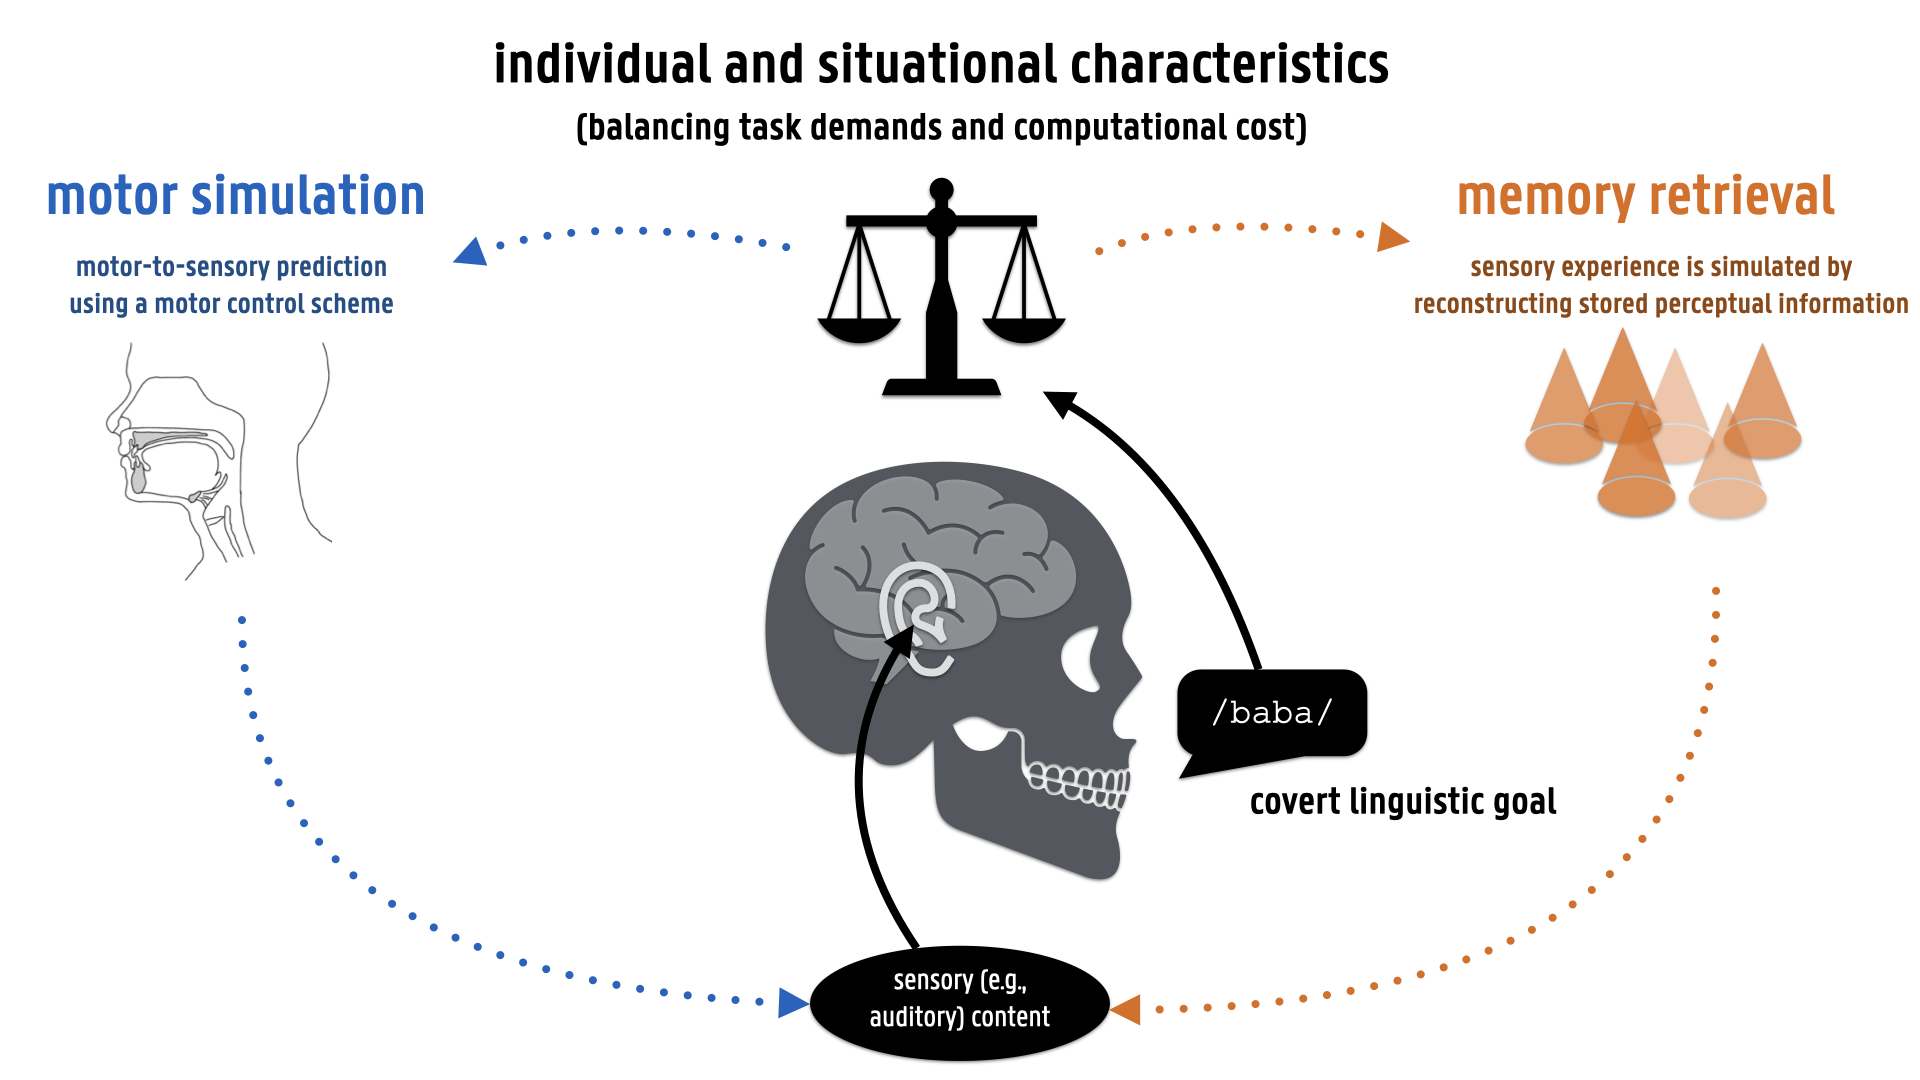
\includegraphics[width=0.75\textwidth]{figures/simulation_association.png} % This is a *.eps file
\end{center}
\caption{General depiction of the balance (weighing) between the prediction-by-simulation (in blue) and prediction-by-association (in orange) mechanisms during covert verbal actions depends on both internal (individual) and external (situational) characteristics that jointly determine the computation cost of each option... FIGURE IN PROGRESS.}\label{fig:1}
\end{figure}

\begin{figure}[ht] % float was h! initially
\begin{center}
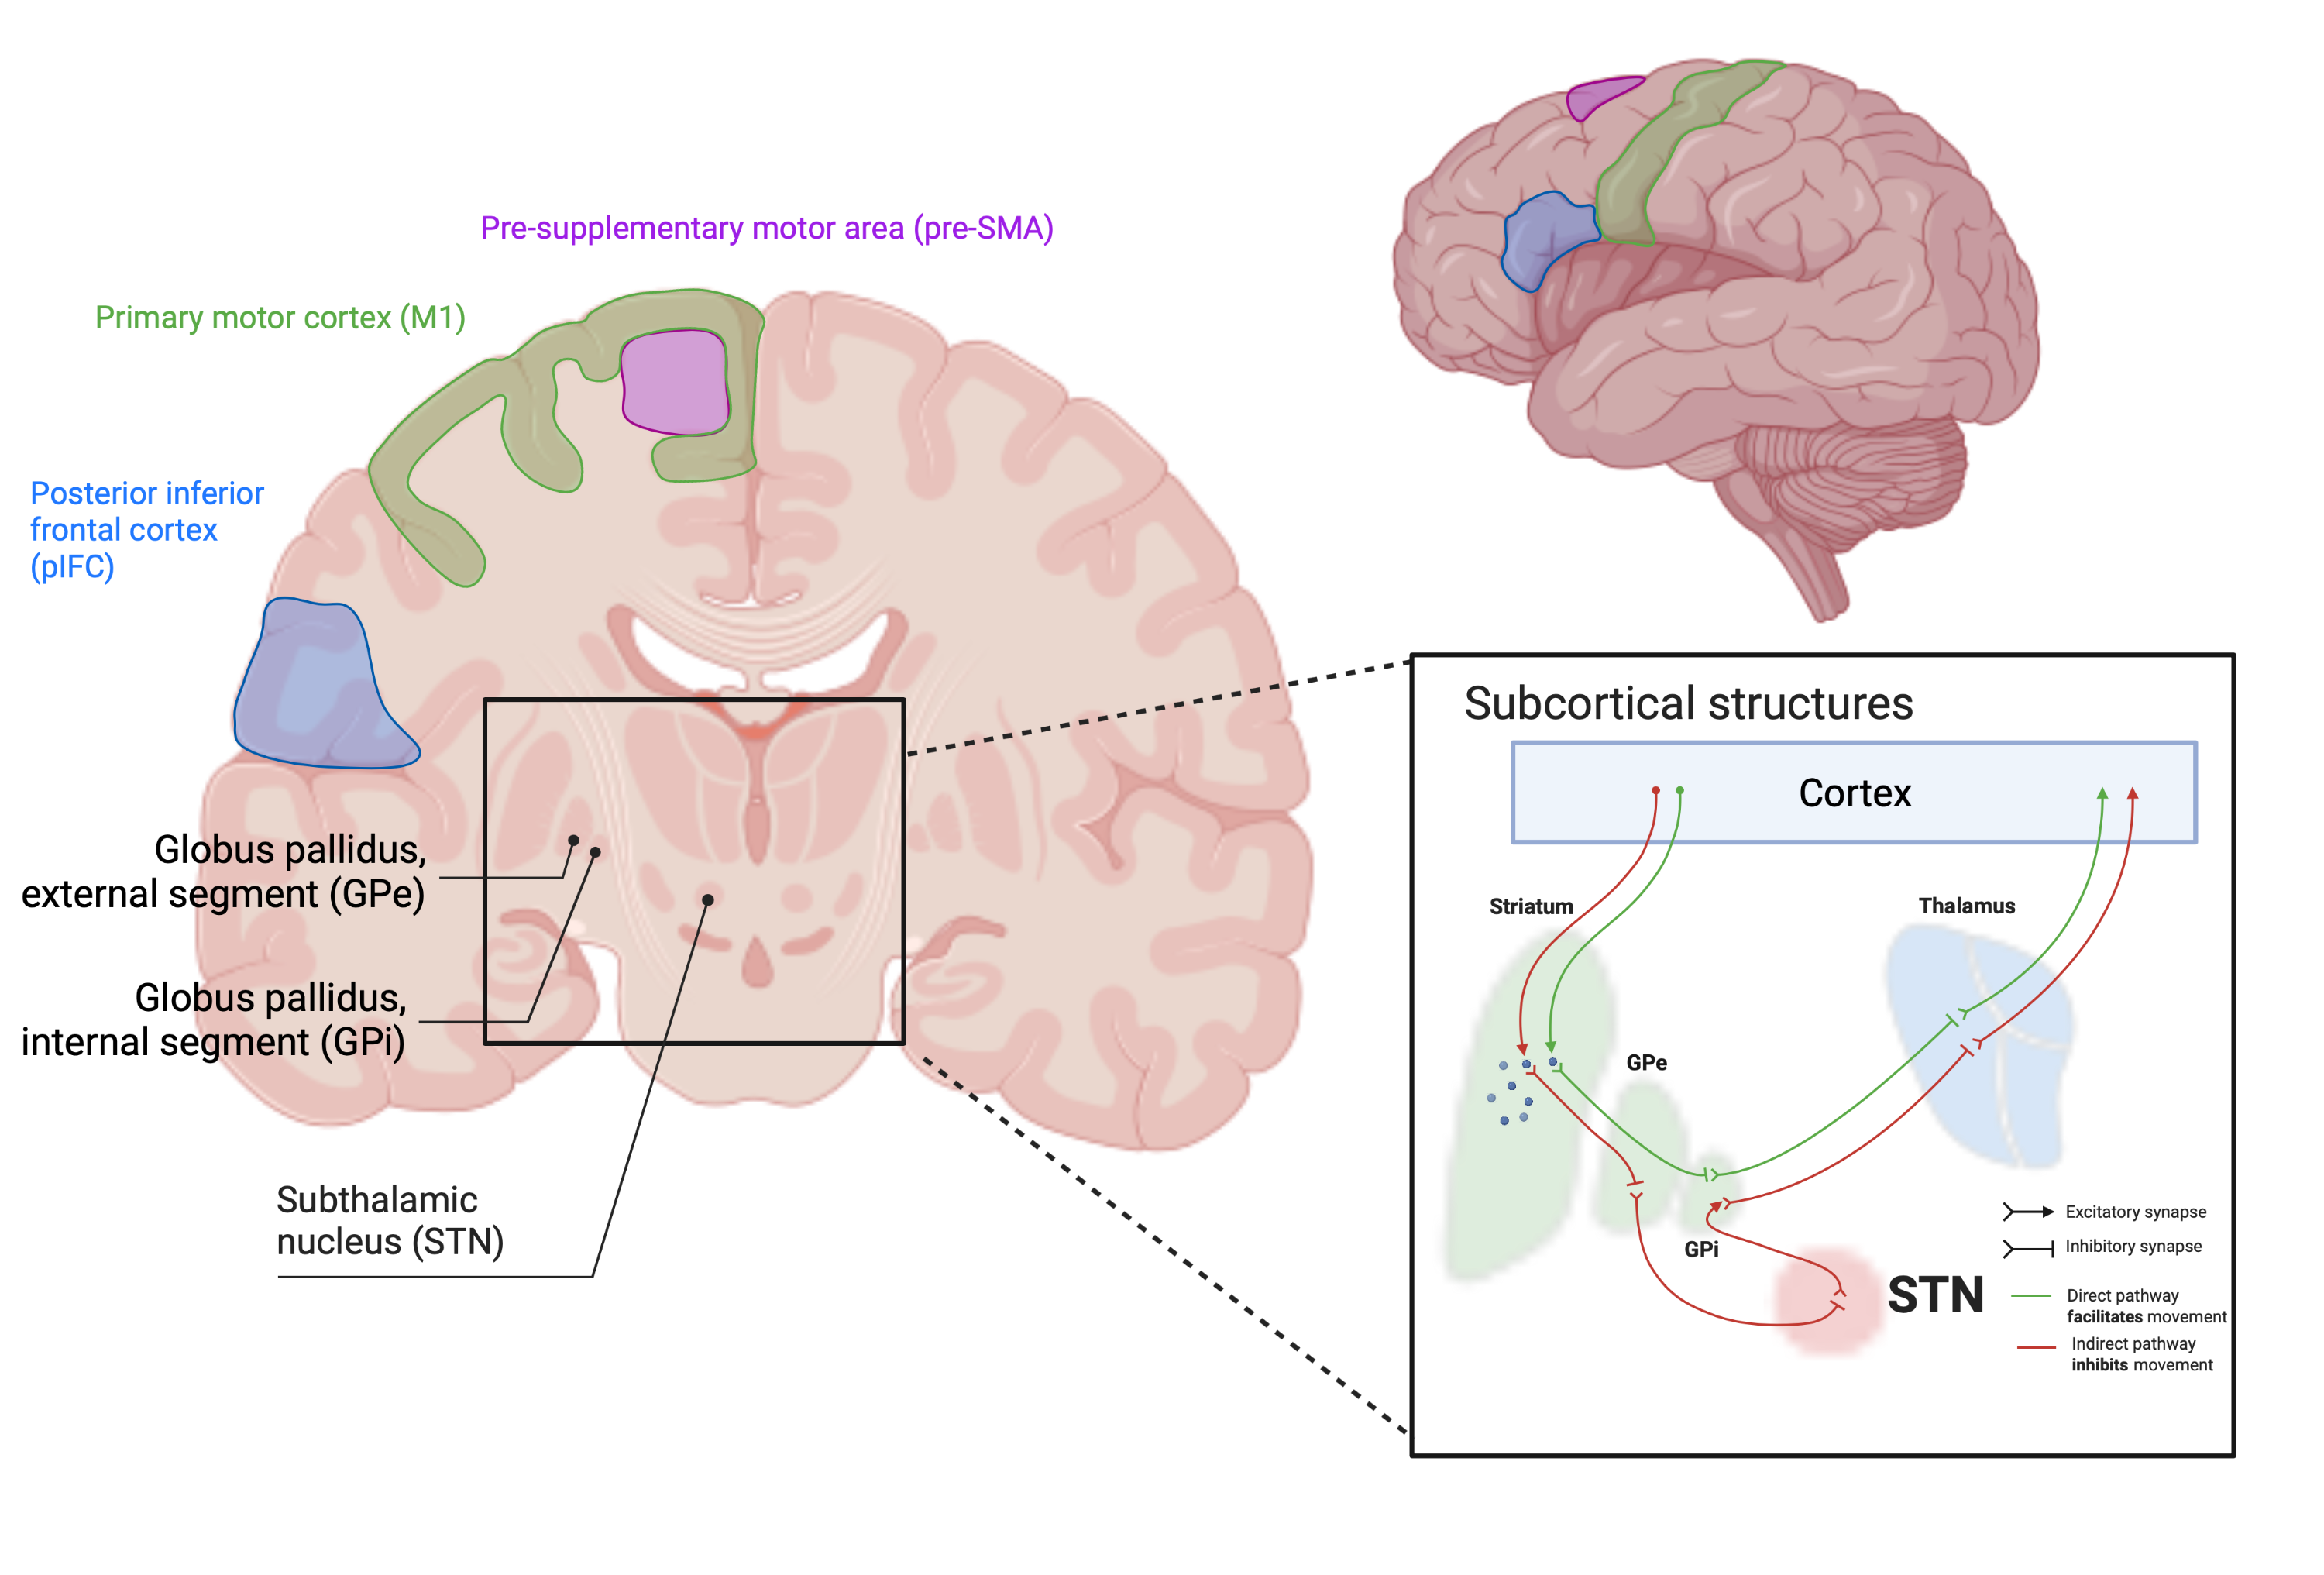
\includegraphics[width=0.75\textwidth]{figures/inhibitory_triangle.png} % This is a *.eps file
\end{center}
\caption{Neural implementation of the inhibitory mechanisms responsible for proactive inhibition during motor imagery. The cerebral complex formed by the preSMA, the rIFC, and the STN is known as the \textit{inhibitory triangle} may be responsible for braking motor commands during covert speech production... FIGURE IN PROGRESS.}\label{fig:2}
\end{figure}

%%% If you are submitting a figure with subfigures please combine these into one image file with part labels integrated.
%%% If you don't add the figures in the LaTeX files, please upload them when submitting the article.
%%% Frontiers will add the figures at the end of the provisional pdf automatically
%%% The use of LaTeX coding to draw Diagrams/Figures/Structures should be avoided. They should be external callouts including graphics.

\end{document}
